\chapter{Исследовательская часть}

В данном разделе будут приведены примеры работы программа, а также проведен сравнительный анализ алгоритмов при различных ситуациях на основе полученных данных.

Технические характеристики устройства, на котором выполнялось тестирование:
\begin{itemize}
	\item операционная система: Windows 11 домашняя;
	\item память: 8 Гбайт;
	\item процессор: Intel(R) Core(TM) i5-10300H CPU @ 2.50ГГц, 2496 МГц, ядер: 4.
\end{itemize}

При тестировании ноутбук был включен в сеть электропитания. Во время тестирования ноутбук не был нагружен сторонними приложениями, которые как-то могли повлиять на результаты тестирования.

\section{Демонстрация работы программы}

На~рисунке~\ref{images:example} приведен пример работы программы.

\begin{figure}[h!]
	\centering
	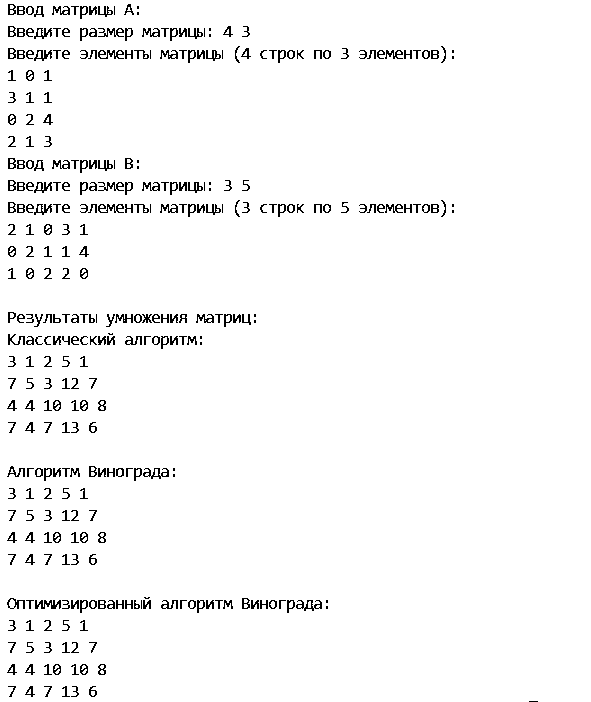
\includegraphics[width=0.5\textwidth]{images/example.png}
	\caption{Пример работы программы}
	\label{images:example}
\end{figure}

\section{Время выполнения реализаций алгоритмов}

В~таблице~\ref{tab:csv} приведены результаты замеров процессорного времени выполнения реализаций алгоритмов умножения матриц.

\begin{table}[H]
	\centering
	\begin{threeparttable}
		\caption{Результаты замеров времени для квадратных матриц}
		\label{tab:csv}
		\csvreader[
		tabular=|c|S|S|S|,
		table head=\hline {Размер} & {Стандартный, мс} & {Виноград, мс} & {Опт. Виноград, мс}\\ \hline,
		late after line=\\ \hline
		]{table/results.csv}{}{
			\csvlinetotablerow
		}
	\end{threeparttable}
\end{table}

По~таблице~\ref{tab:csv} были построены графики представленные на~рисунке~\ref{fig:time_chart}.

\begin{figure}[H]
	\centering
	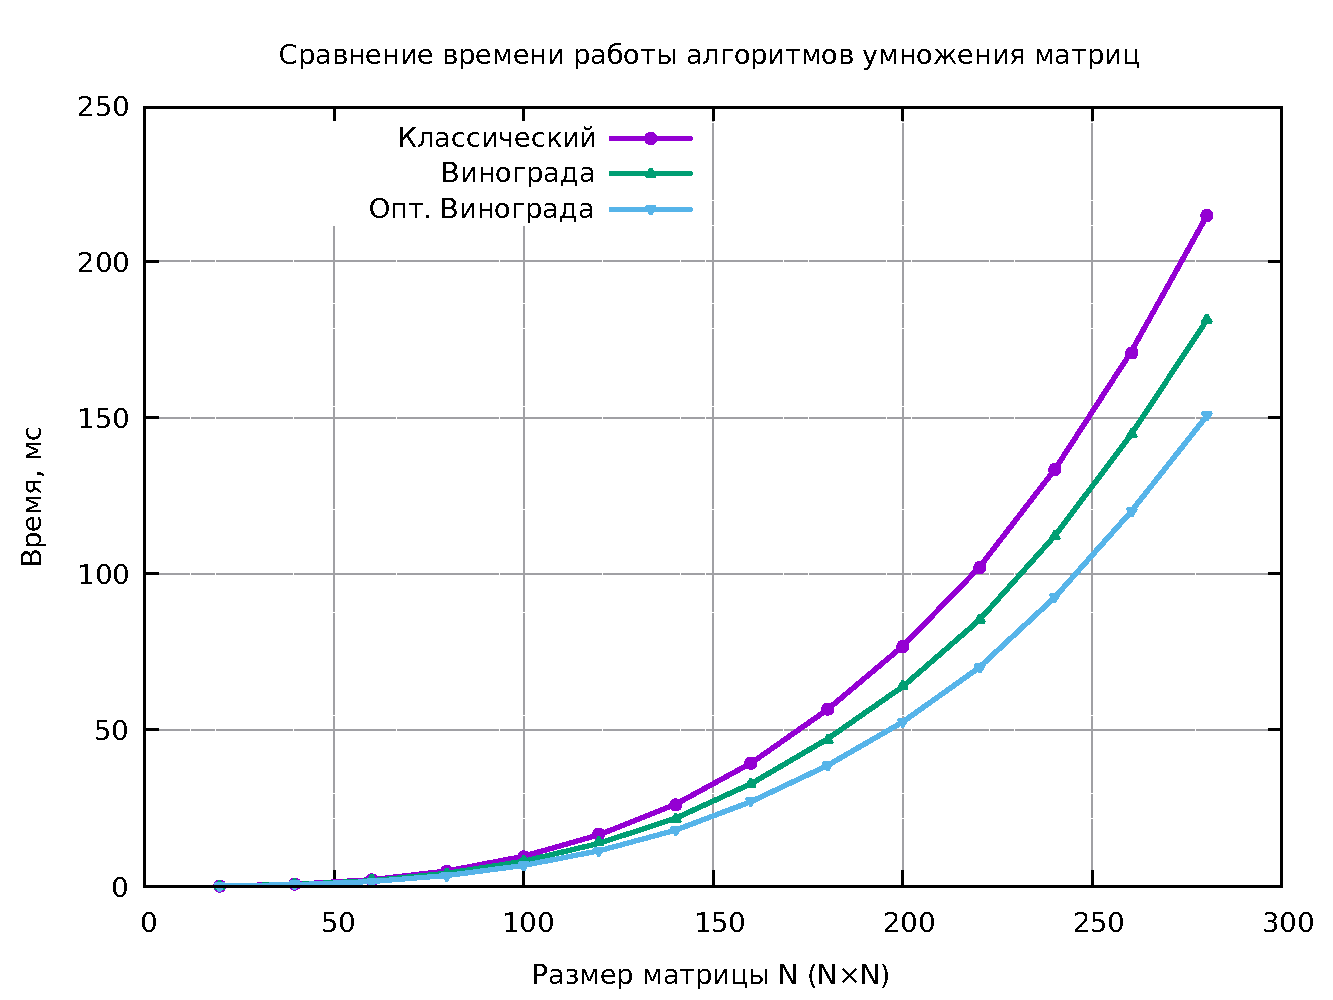
\includegraphics[width=0.8\textwidth]{images/image1.pdf}
	\caption{Графики времени выполнения алгоритмов умножения матриц}
	\label{fig:time_chart}
\end{figure}

\section{Вывод}

Были выполнены замеры процессорного времени для реализаций алгоритмов умножения матриц. Анализ полученных данных показал, что алгоритм Винограда превосходит классический по скорости в 1.09 раза на матрицах размером 10×10 и в 1.20 раза~--- на матрицах 100×100. Оптимизированный алгоритм Винограда демонстрирует ещё большее преимущество, работая быстрее классического на 1.28~---1.46 раза в зависимости от размера матриц.

\clearpage